\section{}
\label{sec:problem1}
%%%%%%%%%%%%%%%%%%%%%%%%%%%%%%%%%%%%%%%%%%%%%%%%%%%%%%%%%%%%%%%%%%%%%%
\paragraph{a)}

For this task, three sets of real data points are studied. The data is loaded from the course web page.

\begin{figure}
    \centering
    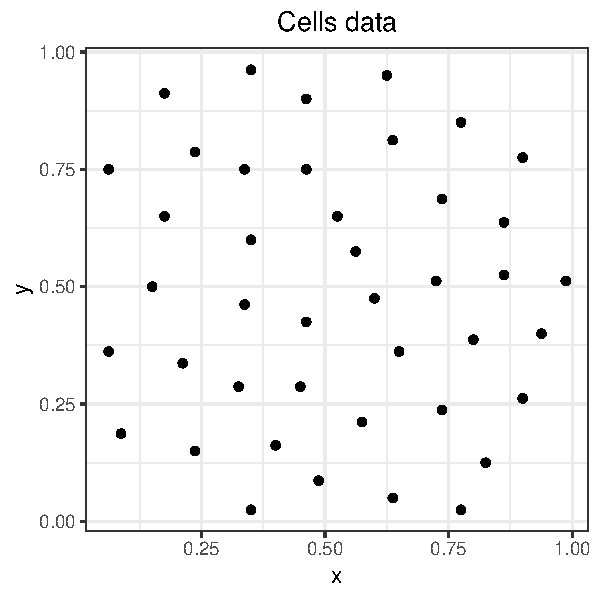
\includegraphics[scale=0.95]{figures/prob1_cells_points.pdf}
    \caption{Data points from \textit{cells.dat}}
    \label{fig:cells_points}
\end{figure}

\begin{figure}
    \centering
    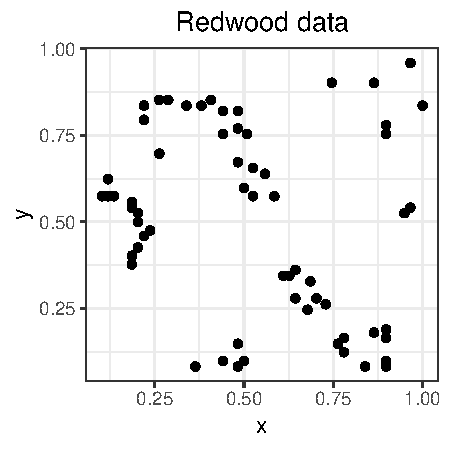
\includegraphics[scale=0.95]{figures/prob1_redwood_points.pdf}
    \caption{Data points from \textit{redwood.dat}}
    \label{fig:redwood_points}
\end{figure}

\begin{figure}
    \centering
    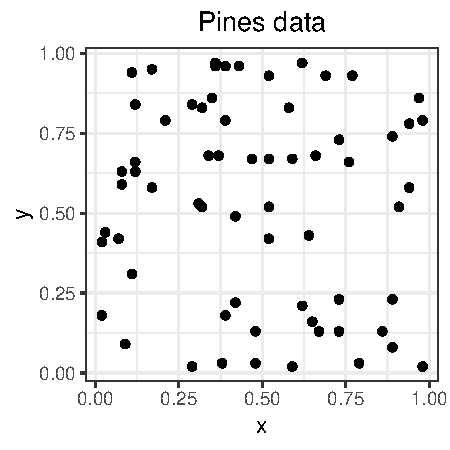
\includegraphics[scale=0.95]{figures/prob1_pines_points.pdf}
    \caption{Data points from \textit{pines.dat}}
    \label{fig:pines_points}
\end{figure}

Figures \ref{fig:cells_points}, \ref{fig:redwood_points} and \ref{fig:pines_points} show the three different data point patterns. These patterns have different properties. The \textit{Pines} data points in Figure \ref{fig:pines_points} seem to be scattered around at random; some close together and some further away without any particular trend. This would happen if the seeds from the trees are spread with the wind somewhat at random, so that some will end up close together and others far apart. The \textit{Redwood} data points (Figure \ref{fig:redwood_points}) are more clustered. This is actually a known feature for redwood trees, as baby redwoods often grow on top of the roots of their parents to get nutrients \footnote{https://www.livescience.com/39461-sequoias-redwood-trees.html}. The \textit{Cells data} (Figure \ref{fig:cells_points}) on the other hand, show the exact opposite property. The points seem to be spread out to max out the space for each cell points, i.e. there seem to be a repulsive effect. The cell-cell repulsion seem to be a true phenomenon due to some proteins. It is an effect that cancer cells lose in contact with normal cells, making them settle down and grow over the normal cells \footnote{https://www.genengnews.com/topics/translational-medicine/mystery-of-cell-cell-repulsion-solved/}

%%%%%%%%%%%%%%%%%%%%%%%%%%%%%%%%%%%%%%%%%%%%%%%%%%%%%%%%%%%%%%%%%%%%%%
\paragraph{b)}

$J(t)$ is an interaction function related to the distance from an event $\vect{x_0}$ to nearby events. Let $\textrm{B}_{x_0}(t)$ be the ball with center in $\vect{x_0}$ and radius $t \geq 0$. Then the number of events inside $\textrm{B}_{x_0}(t)$ is $k_{\textrm{B}_{x_0}(t)}$ and
\begin{equation}
    J(t) = \frac{\E{[k_{\textrm{B}_{x_0}(t)}-1]}}{|\textrm{B}_{x_0}(t) \cap \textrm{D}|}.
\end{equation}
The $-1$ corrects for the event $\vect{x_0}$ already known to be inside the ball. For a stationary Poisson Random Field, the expected number of events inside an subdomain of D is the intensity $\lambda_k$ times the area of the subdomain, since the intensity is constant over the whole domain. Thus, for a stationary Poisson RF, 
\begin{equation}
    J(t) = \frac{\lambda_k |\textrm{B}_{x_0}(t) \cap \textrm{D}|}{|\textrm{B}_{x_0}(t) \cap \textrm{D}|} = \lambda_k.
\end{equation}

Another alternative for evaluating the interaction is using the L-interactive function. For domains in $\R^2$, this is

\begin{equation}
    L(t) = \left[\frac{\E{[k_{\textrm{B}_{x_0}(t)}-1]}}{\lambda_k \pi}\right]^{1/2} = \left[\frac{J(t)|\textrm{B}_{x_0}(t) \cap \textrm{D}|}{\lambda_k \pi}\right]^{1/2}.
\end{equation}

Ignoring boundary effects, that is assuming $|\textrm{B}_{x_0}(t) \cap \textrm{D}| = |\textrm{B}_{x_0}(t)| = \pi t^2$, 
\begin{equation}
    L(t) = \left[\frac{J(t)\pi t^2}{\lambda_k \pi}\right]^{1/2} = \sqrt{\frac{J(t)}{\lambda_k}}t .
    \label{eq:L_function}
\end{equation}

Inserting for $J(t)$ we get that for stationary Poisson RF
\begin{equation}
    L(t) = t
\end{equation}

In R, the empirical L-interaction function can be found using the function Kfn() from the library \textit{spatial}. The empirical L-function for the three data sets are shown in Figure \ref{fig:L_emp}. The plots follow more or less the same straight line for intermediate distances, but for large and in particular for small distances, the functions are somewhat different. The \textit{Cells data} seem to have little interaction at small distances, but has the highest at large distances. The \textit{Redwood data}, on the other hand, seem to have higher interaction at small distances. This fits with the observations from problem 1a) that the \textit{Redwood data} seemed to be more clustered than the others and the \textit{Cells data} more repulsive. 

\begin{figure}
    \centering
    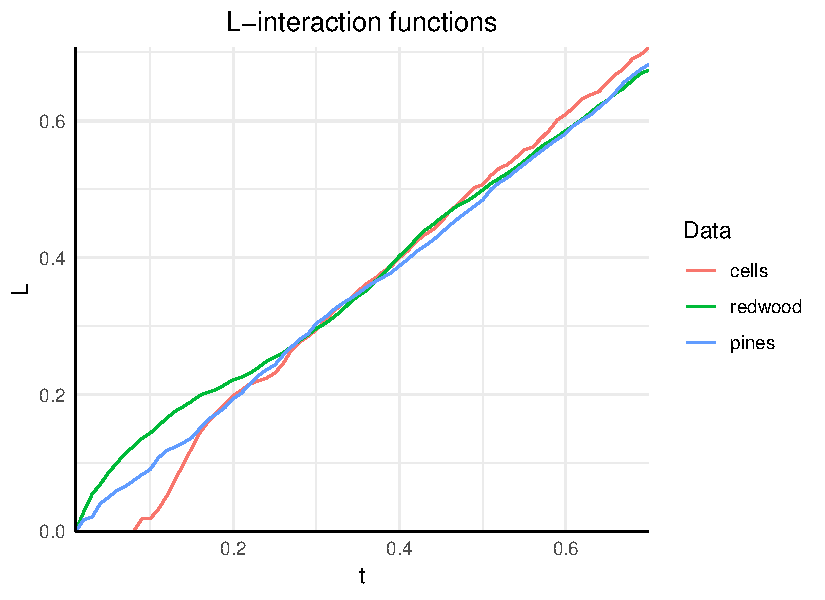
\includegraphics[scale=0.95]{figures/prob1_L_empirical.pdf}
    \caption{Empirical L-interaction functions for the three data sets.}
    \label{fig:L_emp}
\end{figure}

If a stationary Poisson RF is a good model for the data sets, then the empirical L-function should approximately follow $L(t) = t$. In Figure \ref{fig:L_emp_theor}, the empirical interactive functions are plotted against this line. Here, deviation from the line at small distances for the \textit{cells data} and the \textit{redwood data} becomes maybe even more apparent. The \textit{pines data} follows the pretty well, though there is some deviation for larger distances. 

\begin{figure}
    \centering
    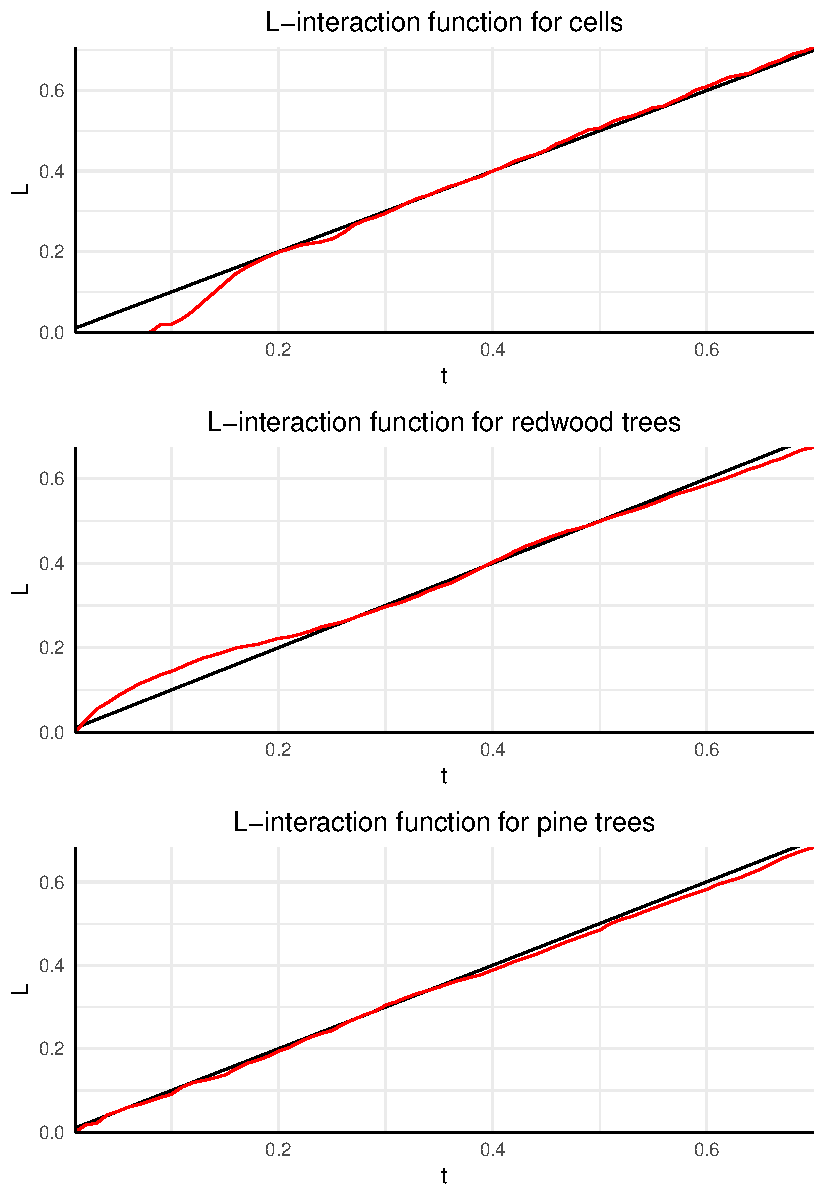
\includegraphics[scale=0.95]{figures/prob1_L_emp_theor.pdf}
    \caption{Empirical L-interaction functions for the three data sets (black lines) plotted against the theoretical (red lines). If a stationary Poisson RF is a suitable model, the red and black lines should more or less overlap.}
    \label{fig:L_emp_theor}
\end{figure}

It seems that a stationary Poisson model may be suitable for the \textit{Pines data}, but not for the two other data sets. However, empirical data must be expected to deviate somewhat from the theoretical value, and to make a more robust conclusion, a test will be performed.

%%%%%%%%%%%%%%%%%%%%%%%%%%%%%%%%%%%%%%%%%%%%%%%%%%%%%%%%%%%%%%%%%%%%%%
\paragraph{c)}
We will now perform an empirical Monte Carlo test to assess whether a stationary Poisson Random Field is a suitable model for each point pattern. This means that we will sample from the distribution of data points under the null hypothesis and qualitatively examine the resulting L-functions. The null hypothesis is that the data origins from a stationary Poisson RF where we have observed all the points. The number of points are $42$ for the \textit{Cells data}, $62$ for the \textit{Redwood data} and $65$ for the \textit{Pines data}.

Under the null hypothesis, conditioning on the number of events, the locations of each event are independent and uniformly distributed in the domain. The domain for each data set is the square $[0,1] \times [0,1]$, so to generate realizations of the Poisson RF, we can draw $x$-coordinates and $y$-coordinates from a uniform (0,1)-distribution. For each data set we draw $100$ realizations with the same amount of data points as in the original set. That is, for the \textit{Cells data} we sample $42\cdot 100$ $x$-coordinates and the same amount of $y$-coordinates, uniformly. For each realization, we compute the empirical L-function, and then we compare these to that of the original data set.

If the given data points origin from a stationary Poisson RF, their empirical L-functions should behave approximately as the generated realizations. The L-functions of these realizations, with corresponding empirical $95\%$ and $5\%$ quantiles, are displayed in Figure \ref{fig:poiss_samps}. The same quantiles, making up a $0.9$-interval for each distance $t$, are displayed in Figure \ref{fig:poiss_quantiles} together with the empirical L-function of the original data points.

\begin{figure}
    \centering
    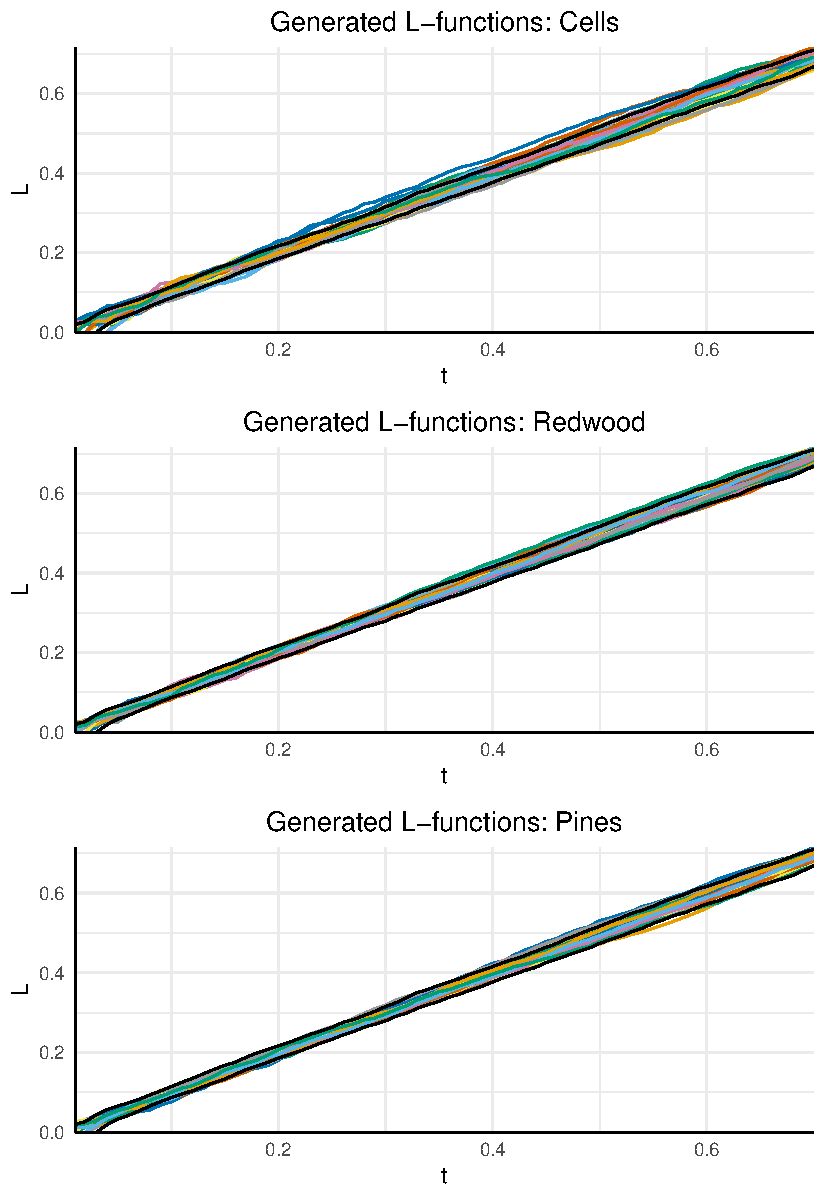
\includegraphics[scale=0.95]{figures/prob1_samples.pdf}
    \caption{}
    \label{fig:poiss_samps}
\end{figure}

\begin{figure}
    \centering
    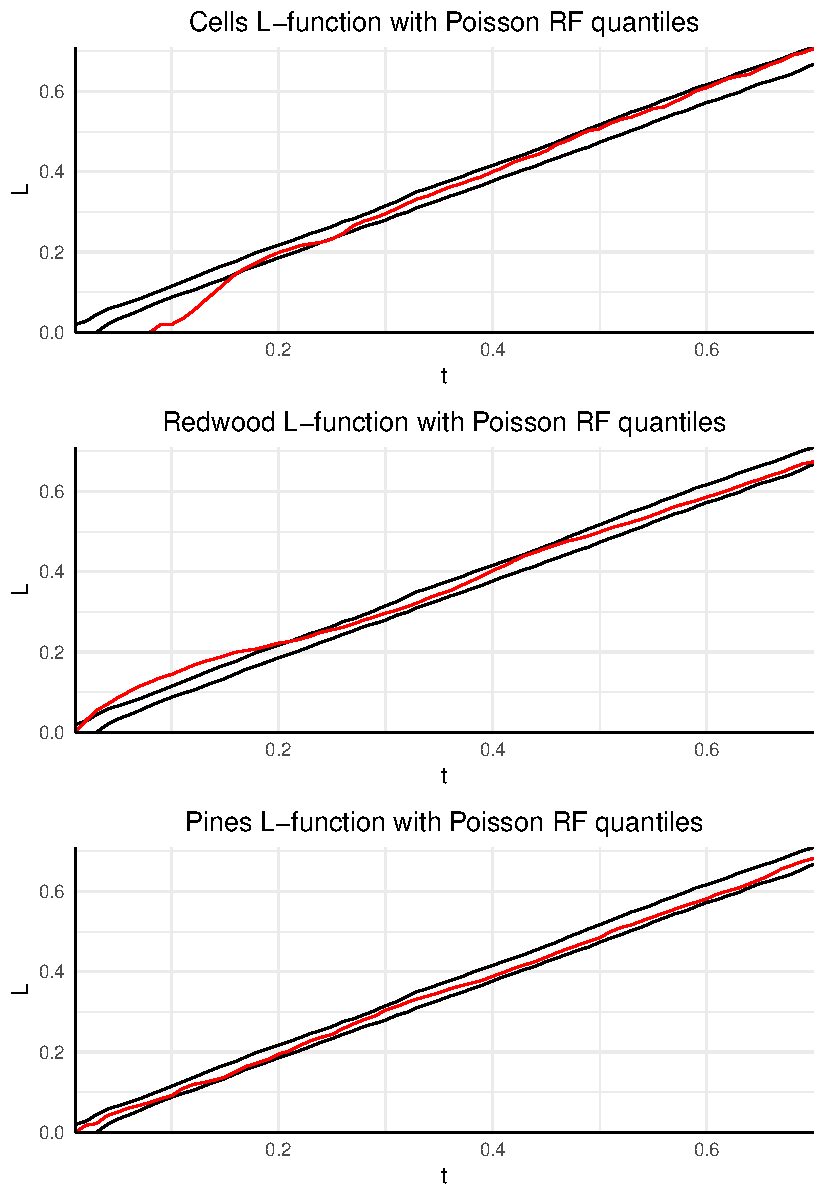
\includegraphics[scale=0.95]{figures/prob1_quantiles.pdf}
    \caption{}
    \label{fig:poiss_quantiles}
\end{figure}

Thus for each given distance computed by Kfn(), the empirical $0.9$ confidence interval tells us that approximately $90\%$ of all empirical L-functions that are made from stationary Poisson RFs (with the given amount of observed data points) will lay within this interval at this distance. Confidence intervals and hypothesis tests are connected, and another way of assessing the interval is that given that if the original data points origin from a Poisson RF, then for each distance given by the Kfn() function, the empirical L-function will only be outside the interval with probability of $0.1$. In Figure \ref{fig:poiss_quantiles}, that for small distances, the L-functions for the \textit{Redwood data} and, in particular, the \textit{Cells data} lay pretty far outside their respective intervals. For large distances, there L-functions do not deviate much from what would be expected, but it makes sense that repulsion and clustering will have the most effect on the number of neighboring events for small distances.

We could extend the quantiles to $0.01$ and $0.99$ to make approximate $98\%$ confidence intervals. Figure \ref{fig:poiss_quantiles2} show the area of interest for the \textit{Cells data} and the \textit{Redwood data}. There is only a probability of about $0.01$ to be at either side of the intervals for each $t$. With the clear deviation that we can see in Figure \ref{fig:poiss_quantiles2}, we conclude that this hypothesis should be rejected, and thus that a Poisson is not a suitable model for the \textit{Cells data} and the \textit{Redwood data}. For these, the Neuman-Scott cluster model and the Strauss repulsion model will be used instead for the two data sets, respectively. These will be assessed in Problems 3 and 4. 

\begin{figure}
    \centering
    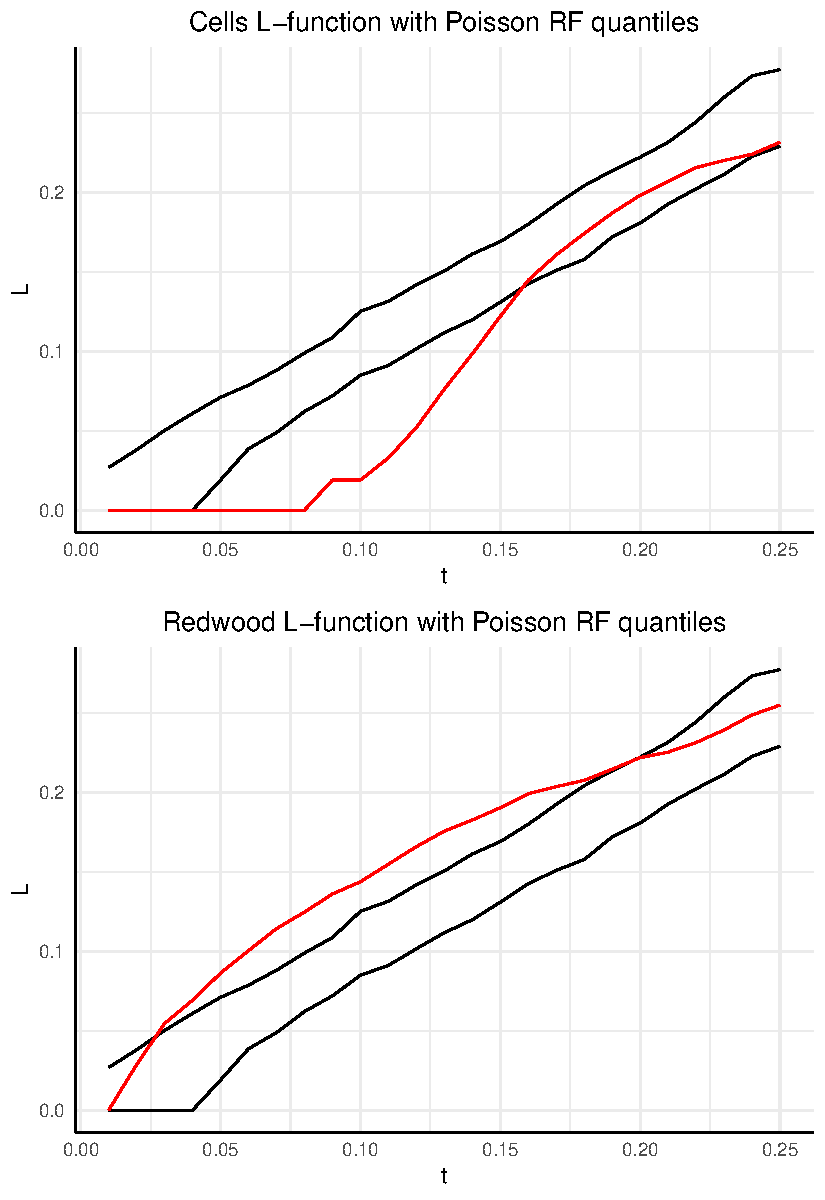
\includegraphics[scale=0.95]{figures/prob1_quantiles2.pdf}
    \caption{}
    \label{fig:poiss_quantiles2}
\end{figure}

The \textit{Pines data} L-function lays within or on the limits of the $0.9$ interval for all distances, and seem to follow a similar pattern as the generated Pines realizations in figure \ref{fig:poiss_samps}. Thus, we conclude that a Poisson RF is a suitable model for this data.